\documentclass[11pt]{article}
\usepackage{graphicx}
\usepackage{amsmath}
\usepackage{hyperref}
\usepackage{listings}
\usepackage{xcolor}
\usepackage{circuitikz}


\topmargin=-0.45in
\evensidemargin=0in
\oddsidemargin=0in
\textwidth=6.5in
\textheight=9.0in
\headsep=0.25in
\renewcommand{\thesubsection}{\alph{subsection})}
\renewcommand\lstlistingname{Snippet}
\renewcommand\lstlistlistingname{}

\usepackage{xcolor}
\definecolor{codegreen}{rgb}{0,0.6,0}
\definecolor{codegray}{rgb}{0.5,0.5,0.5}
\definecolor{codeorange}{rgb}{1,0.49,0}
\definecolor{backcolour}{rgb}{0.95,0.95,0.96}

\lstdefinestyle{mystyle}{
    backgroundcolor=\color{backcolour},   
    commentstyle=\color{codegray},
    keywordstyle=\color{codeorange},
    numberstyle=\tiny\color{codegray},
    stringstyle=\color{codegreen},
    basicstyle=\ttfamily\footnotesize,
    breakatwhitespace=false,         
    breaklines=true,                 
    captionpos=b,                    
    keepspaces=true,                 
    numbers=left,                    
    numbersep=5pt,                  
    showspaces=false,                
    showstringspaces=false,
    showtabs=false,                  
    tabsize=2,
    xleftmargin=10pt,
}

\lstset{style=mystyle}
% Title and Author Customization

% --------------------
% Start from here
% --------------------

\title{
    \vspace{3em}
    \textbf{Digital Signal Processing Lab}\\
    Demo 8 - Exercise 1 (Echo system)
    \vspace{1em}
}
\author{
    Saad Zubairi \\ 
    shz2020 \\
    \vspace{1em}
}
\vspace{1em}
\date{September 17th, 2025}

\begin{document}
\maketitle	

\pagebreak

% --------------------
% Body
% --------------------


\section{Difference Equation}

From the code:

$$
y(n)= b_{0}x(n) + Gx(n-N)
$$

with $b_{0} = 1.0$, $G=0.8$, and $ N =$ the delay in samples.

\section{Transfer Function}

Take the Z-transform
$$
Y(z)= b_{0}X(z) + Gz^{-N}X(z)
$$

so the transfer function becomes:
$$
H(z)=\frac{Y(z)}{X(z)}= b_{0} + Gz^{-N}
$$

\section{Impulse Response}
Impulse response will just be the inverse Z transform of the transfer function, which will be:

$$
h(n)= b_{0}\delta(n) + G\delta(n-N)
$$

The sketch of which is as follows:

(for this example, we'll take a small value of $G=5$)

\bigskip
\begin{tikzpicture}
    % axes
    \draw[->] (0,-0.5) -- (0,3) node[left] {$h[n]$};
    \draw[->] (0,0) -- (9,0) node[right] {$n$};

    % impulses
    \foreach \x in {1,...,8} {
        \draw[thick] (\x,0) -- (\x,0); % default stems at zero
    }

    % actual impulses
    \draw (1,0) -- (1,2) node[above] {$1$} ;
    \draw (6,0) -- (6,1.6) node[above] {$0.8$} ;
    
    % labels
    \foreach \x in {1,...,8} \draw (\x,0) node[below] {\pgfmathparse{\x-1}\pgfmathresult};

\end{tikzpicture}

\section{Pole Zero Plot}

Here's the pole zero plot of this filter:

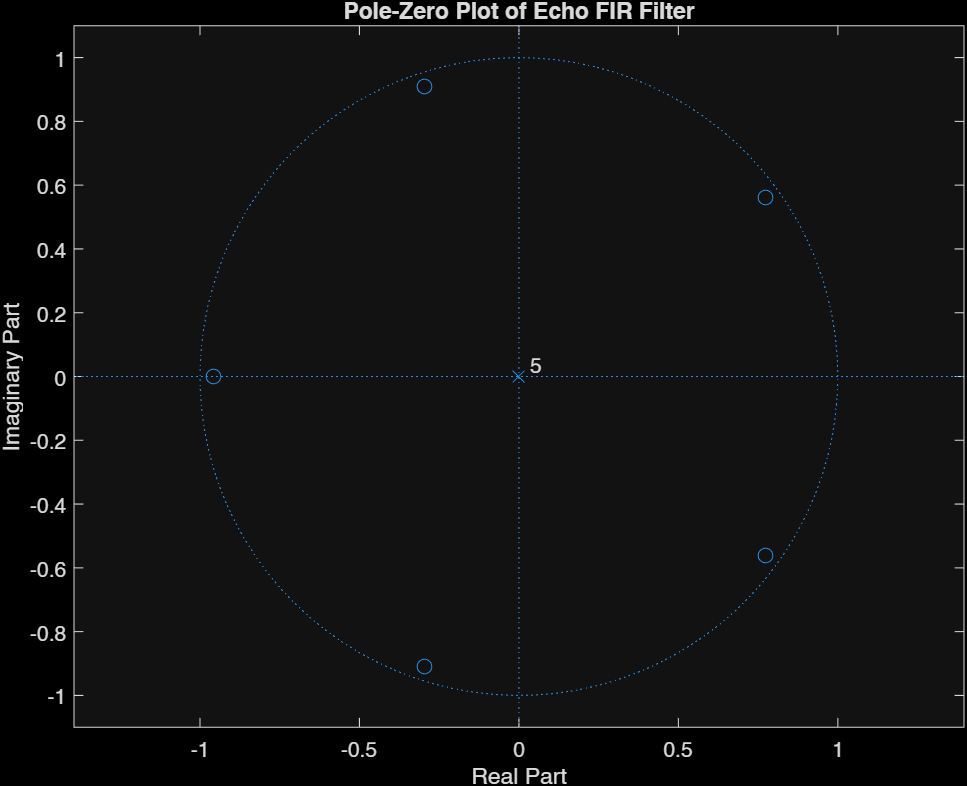
\includegraphics[scale=0.4]{untitled1.png}

\end{document}